%%
%% Template chap2.tex
%%

\chapter{Experiment 1: Learning with Random Sampling}
\label{cha:expt1}

\section{Preparation of Data}


\begin{itemize}
	\item Preparing the SDSS dataset:
	 Obtain data from SkyServer via SQL query (see Appendix for code)
	 \item Preparing the VST ATLAS: Data specifically prepared by Christian Wolf
	\item Convert data to HDF Table for fast reading
\end{itemize}


\section{Experimental Protocol}
\label{sec:protocol1}

SDSS Colour Features
\begin{itemize}
	\item Convert magnitude features to colours. Reason: remove distance dependence.
	Use five colours and one r-band magnitudes -- a rule of thumb used by astronomers.
	Choose r-band since it captures the most light, hence hopefully we have a low
	signal-to-noise ratio
\end{itemize}
Comparing Three sets of reddening correction on SDSS
\begin{itemize}
	\item Split into balanced training set (600,000) and test set (300,000).
	\item Use random forest (fast and accurate) with 300 trees
	\item Compare recall maps and accuracy rates
\end{itemize}
Comparing three families of classifiers: shuffle split with 5 iterations, train size is
up to 300,000 and test size is 200,000.
\begin{itemize}
	\item Random Forest, Logistic Regression, and SVM
	\item Do a grid search to optimise hyperparameters
	\item Plot learning curve with random sampling
	\item Use linear decision boundaries in SVM and Logistic but transform features with
	degree 2 and 3 polynomial.
\end{itemize}
Run random forest on all 2.8 million labelled examples and predict proportion 
on the 800 million unlabelled data. Corrections are made for the potential misclassification.



\section{Results and Discussion}
\label{sec:results1}

\subsection{Comparison of Reddening Correction Sets}
No significant difference. Will use W14 set for reasons stated in \cite{wolf14}.


\begin{figure}[tbp]
	\centering
	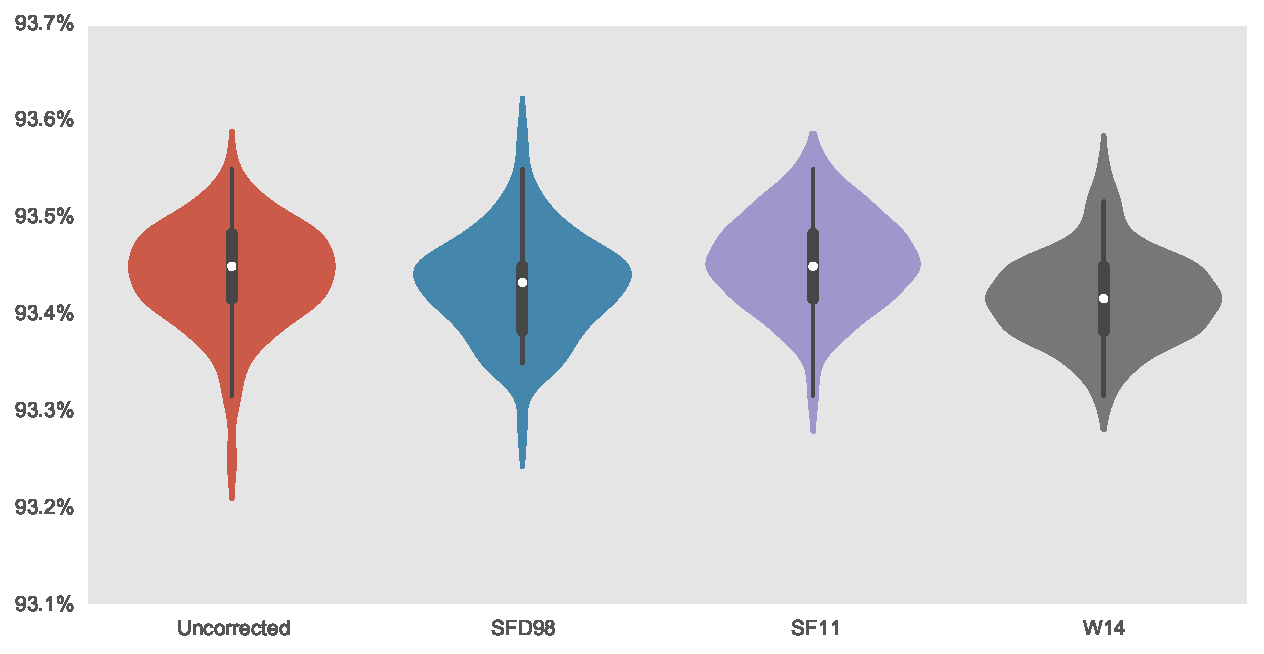
\includegraphics[width=\textwidth]{figures/violin_reddening_correction}
	\caption{Comparing the accuracy rates using 4 correction sets.}
	\label{fig:reddeningviolin}
\end{figure}

\subsection{Learning Curves with Random Sampling}
Optimal Hyper-parameters for SDSS
\begin{itemize}
	\item SVM RBF: $C = 10 000$ and $\gamma = 0.001$.
	\item SVM Polynomial degree 2 with one-vs-rest strategy, squared hinge loss and L1-norm
	(giving us sparse solutions) and $C = 0.1$.
	\item Logistic degree 2 also with one-vs-rest strategy, L1-norm and $C=1$.
\end{itemize}
Learning Curves
\begin{itemize}
	\item Random forest is the fastest and most accurate
	\item Degree 3 polynomial transformation offers better results than degree 2, although
	both do level off after 100,000 examples.
	\item Logistic degree 3 was stopped early as it took too long to run.
\end{itemize}


\begin{figure}[tbp]
	\centering
	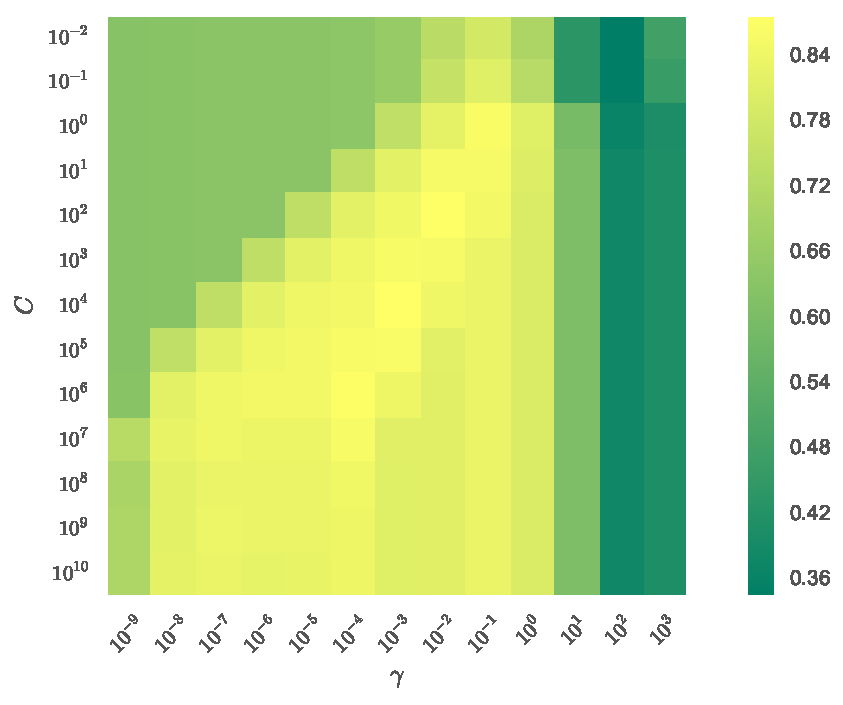
\includegraphics[width=0.7\textwidth]{figures/heat_gridsearch_svm_rbf}
	\caption{Accuracy rate heat map of the hyperparameters of SVM (RBF) for the SDSS.}
	\label{fig:sdss_heat_rbf}
\end{figure}

\begin{figure}[tbp]
	\centering
	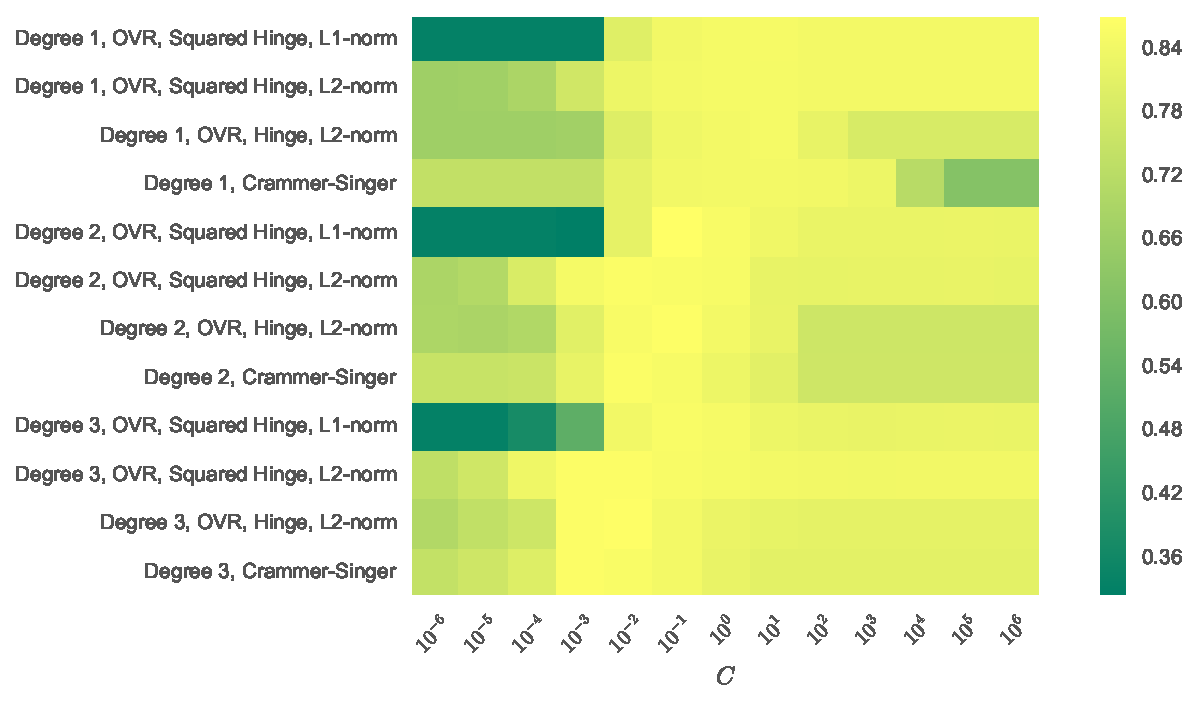
\includegraphics[width=\textwidth]{figures/heat_gridsearch_svm_poly}
	\caption{Accuracy rate heat map of the hyperparameters of SVM (Polynomial) for the SDSS.}
	\label{fig:sdss_heat_poly}
\end{figure}

\begin{figure}[tbp]
	\centering
	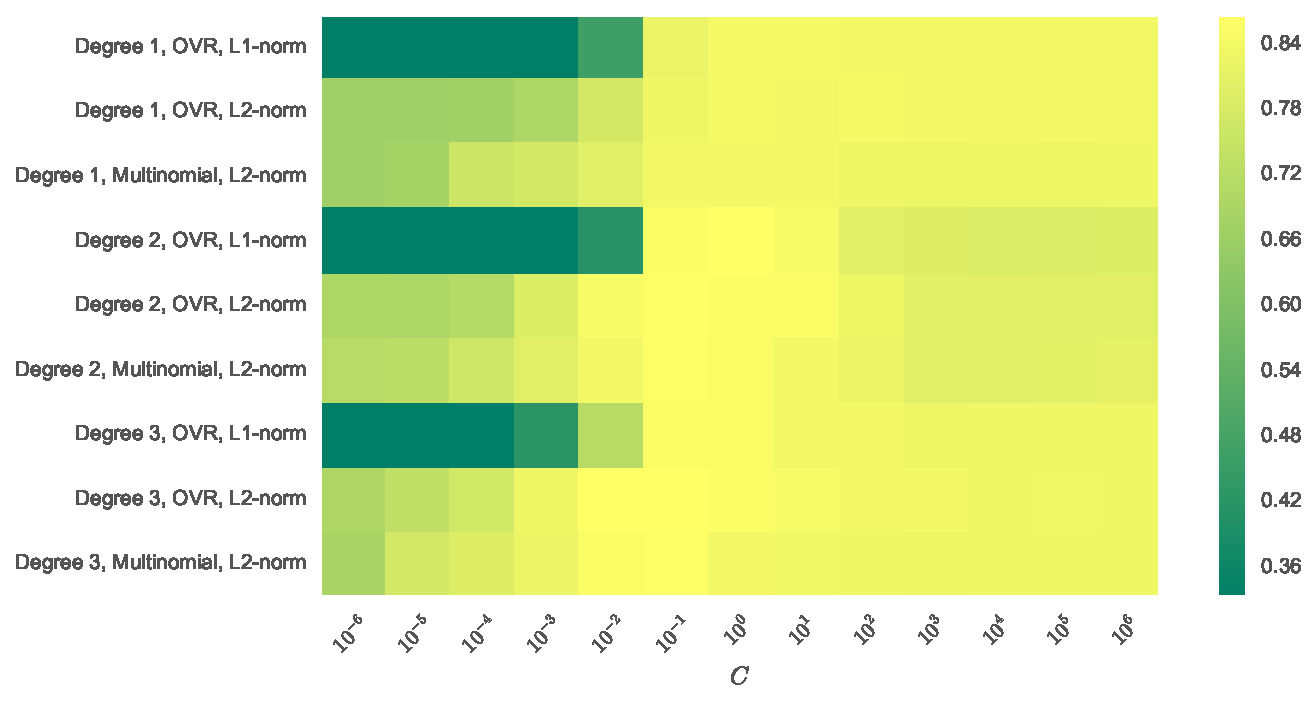
\includegraphics[width=\textwidth]{figures/heat_gridsearch_logistic}
	\caption{Accuracy rate heat map of the hyperparameters of Logistic Regression for the SDSS.}
	\label{fig:sdss_heat_logistic}
\end{figure}

\begin{figure}[tbp]
	\centering
	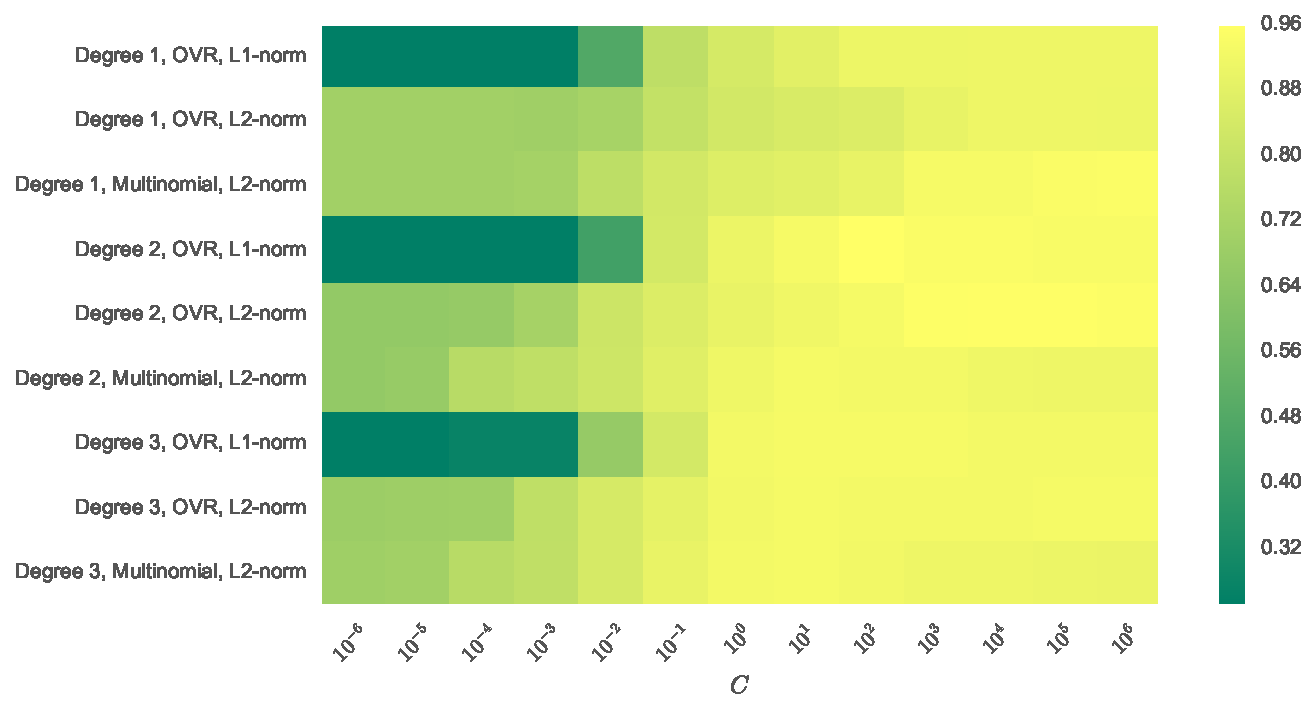
\includegraphics[width=\textwidth]{figures/heat_vstatlas_vgridsearch_logistic}
	\caption{Accuracy rate heat map of the hyperparameters of Logistic Regression for the VST ATLAS.}
	\label{fig:vst_heat_logistic}
\end{figure}


\begin{figure}[tbp]
	\centering
	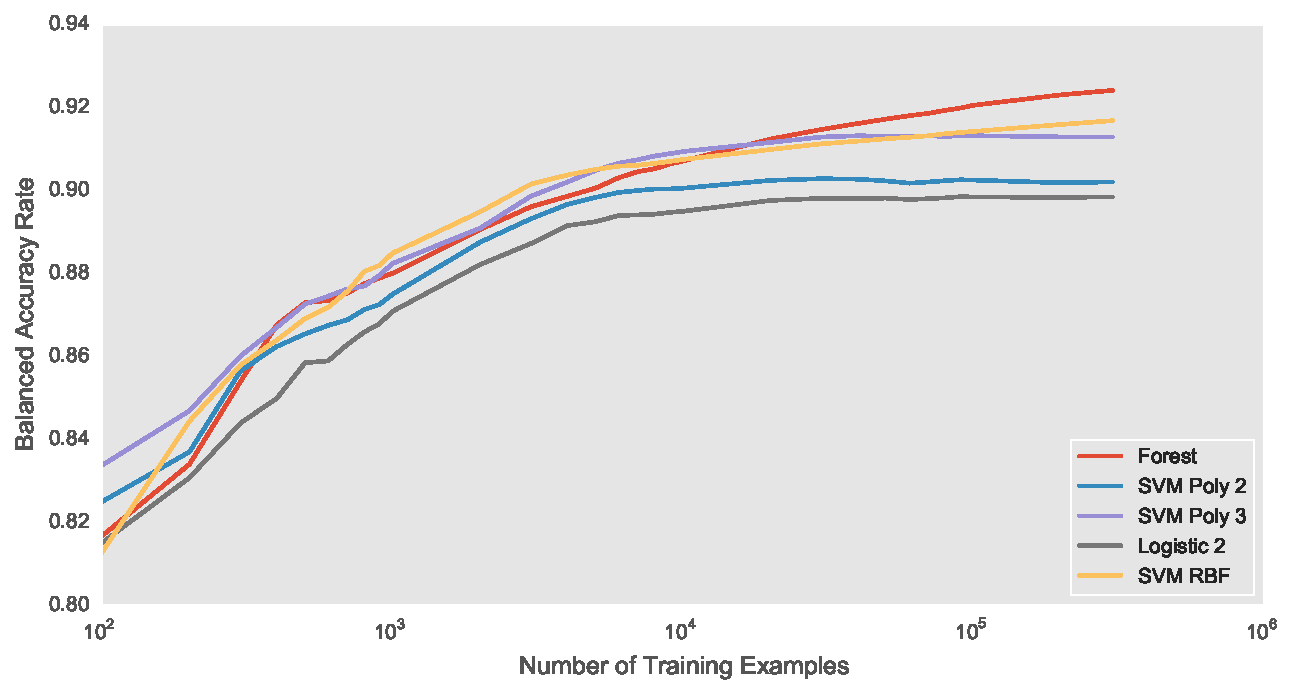
\includegraphics[width=\textwidth]{figures/learning_curves_sdss_random}
	\caption{SDSS learning curves with random sampling.}
	\label{fig:sdss_learning}
\end{figure}





\subsection{Class Proportion Estimation}
See Figure \ref{fig:forest} for predictions. Show confusion matrix, and
both uncorrected and corrected values.
\begin{figure}[p]
	\centering
	\begin{subfigure}{\textwidth}
		\centering
		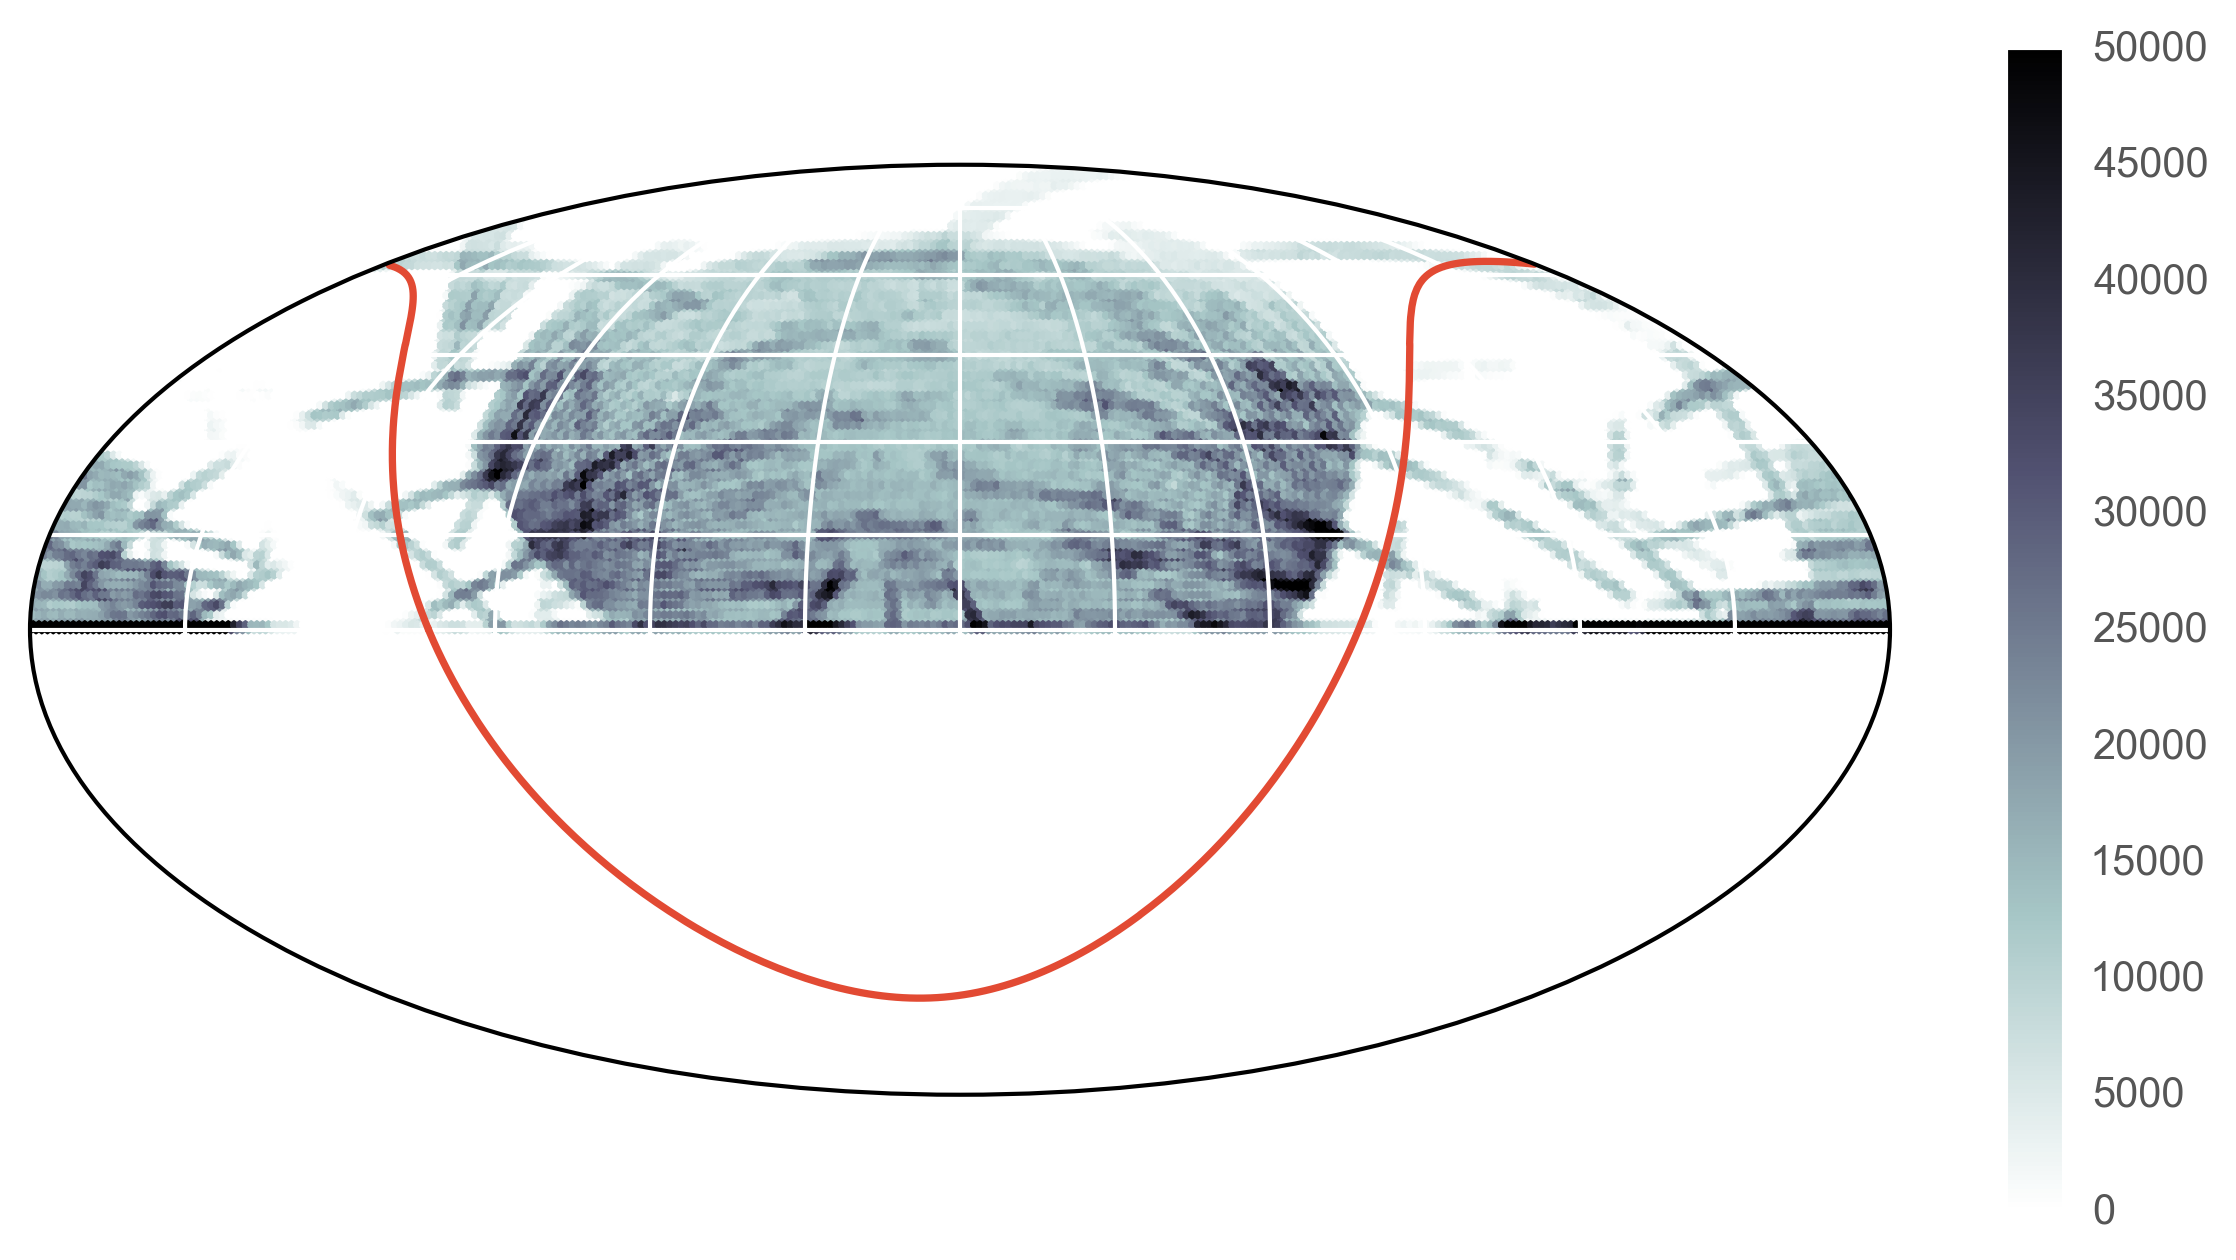
\includegraphics[width=0.75\textwidth]{figures/map_prediction_forest_galaxies}
		\caption{Distribution of galaxies.}
		\label{fig:random1}
	\end{subfigure}\\
	\begin{subfigure}{\textwidth}
		\centering
		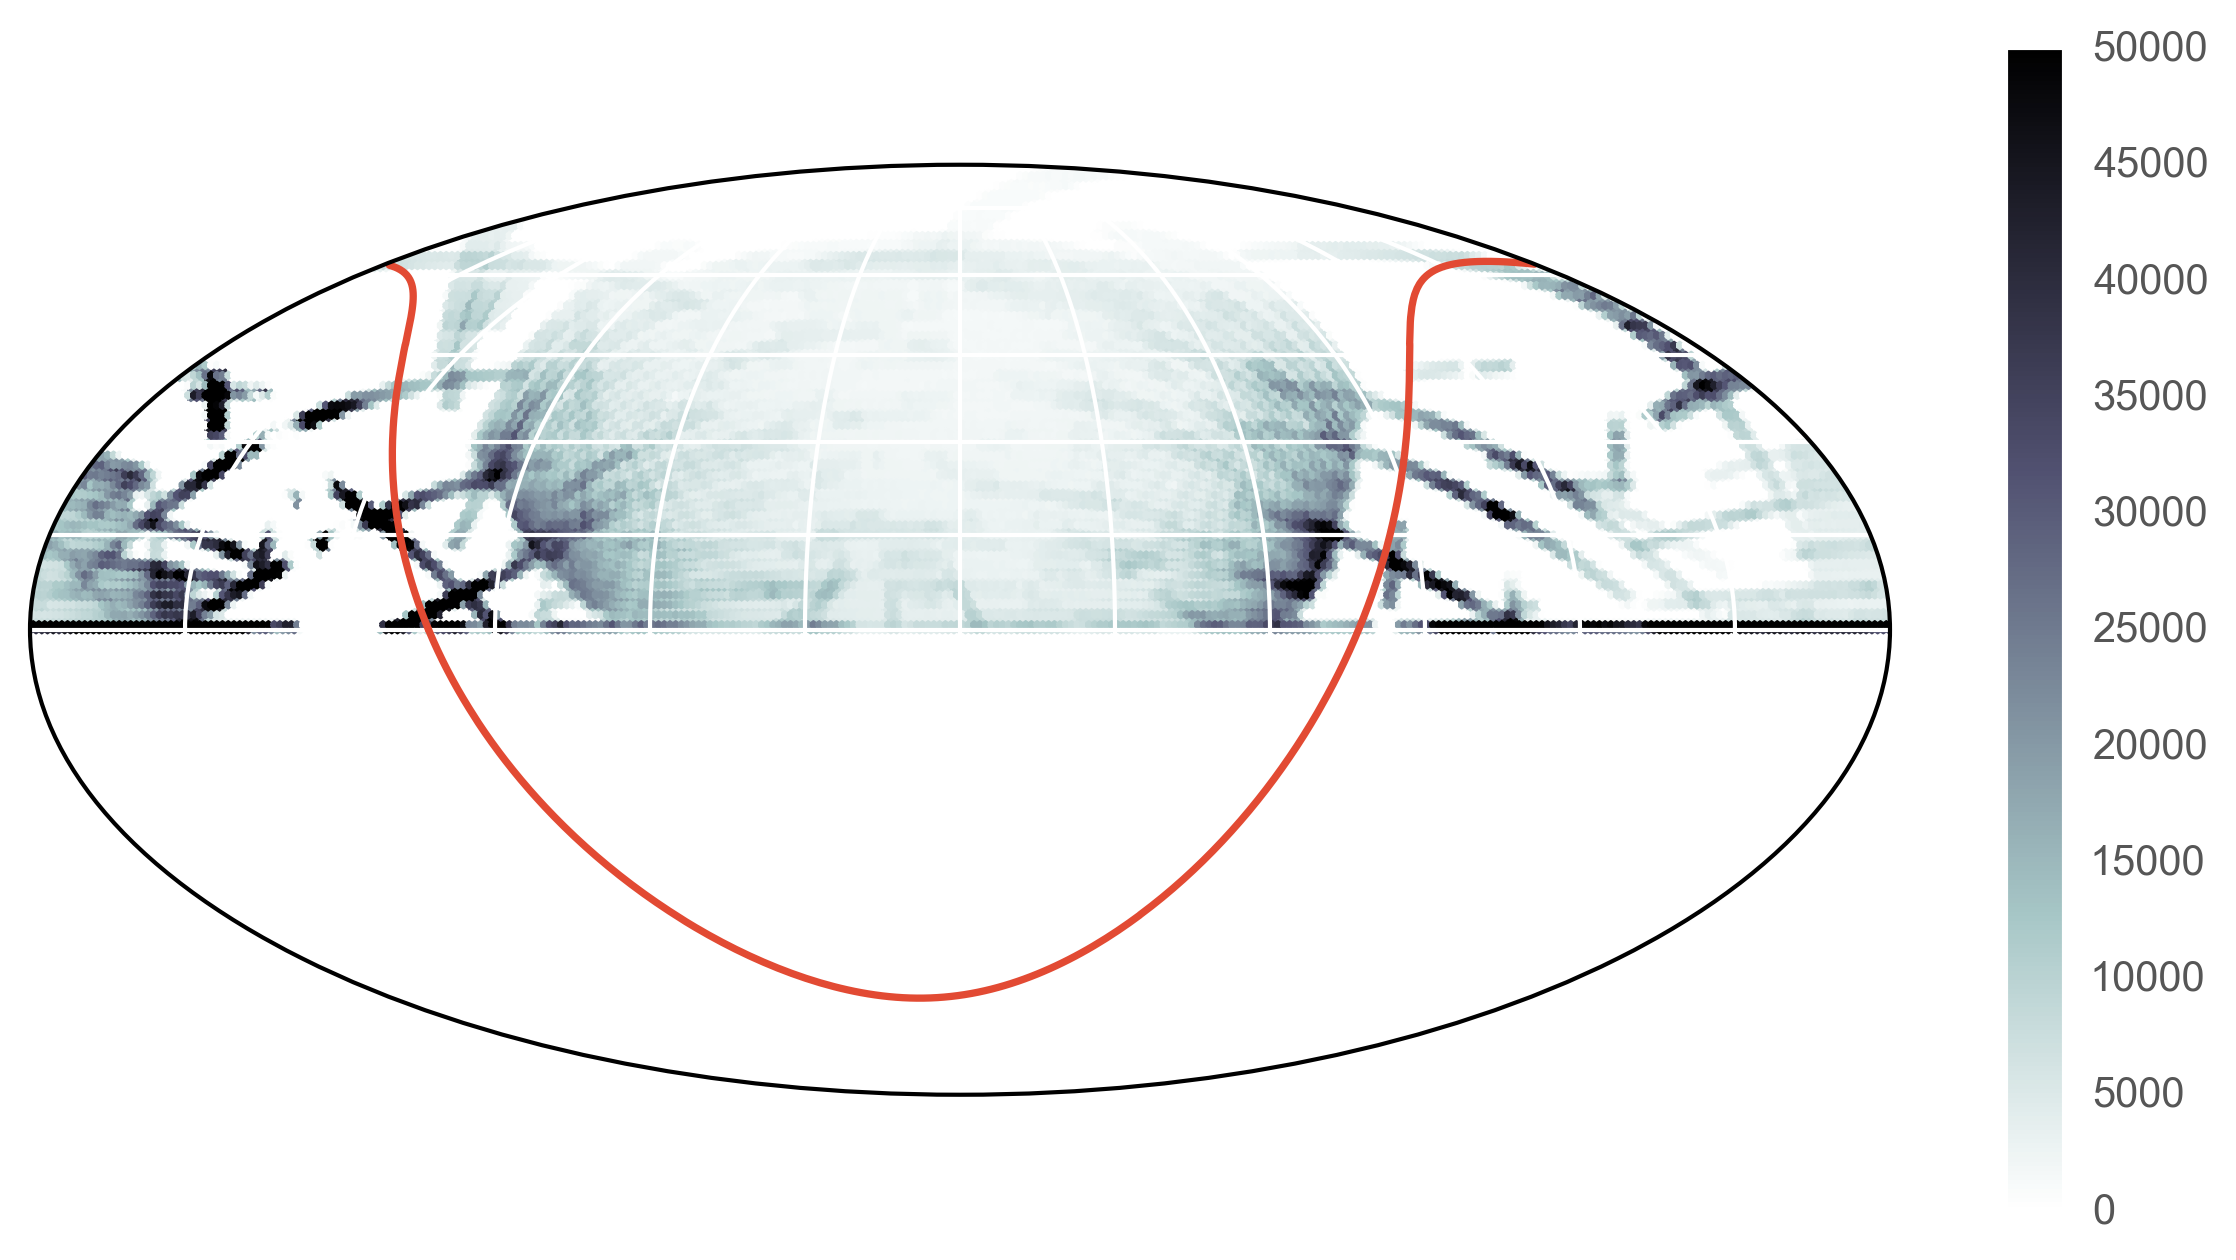
\includegraphics[width=0.75\linewidth]{figures/map_prediction_forest_stars}
		\caption{Distribution of stars.}
		\label{fig:random2}
	\end{subfigure}
	\begin{subfigure}{\textwidth}
		\centering
		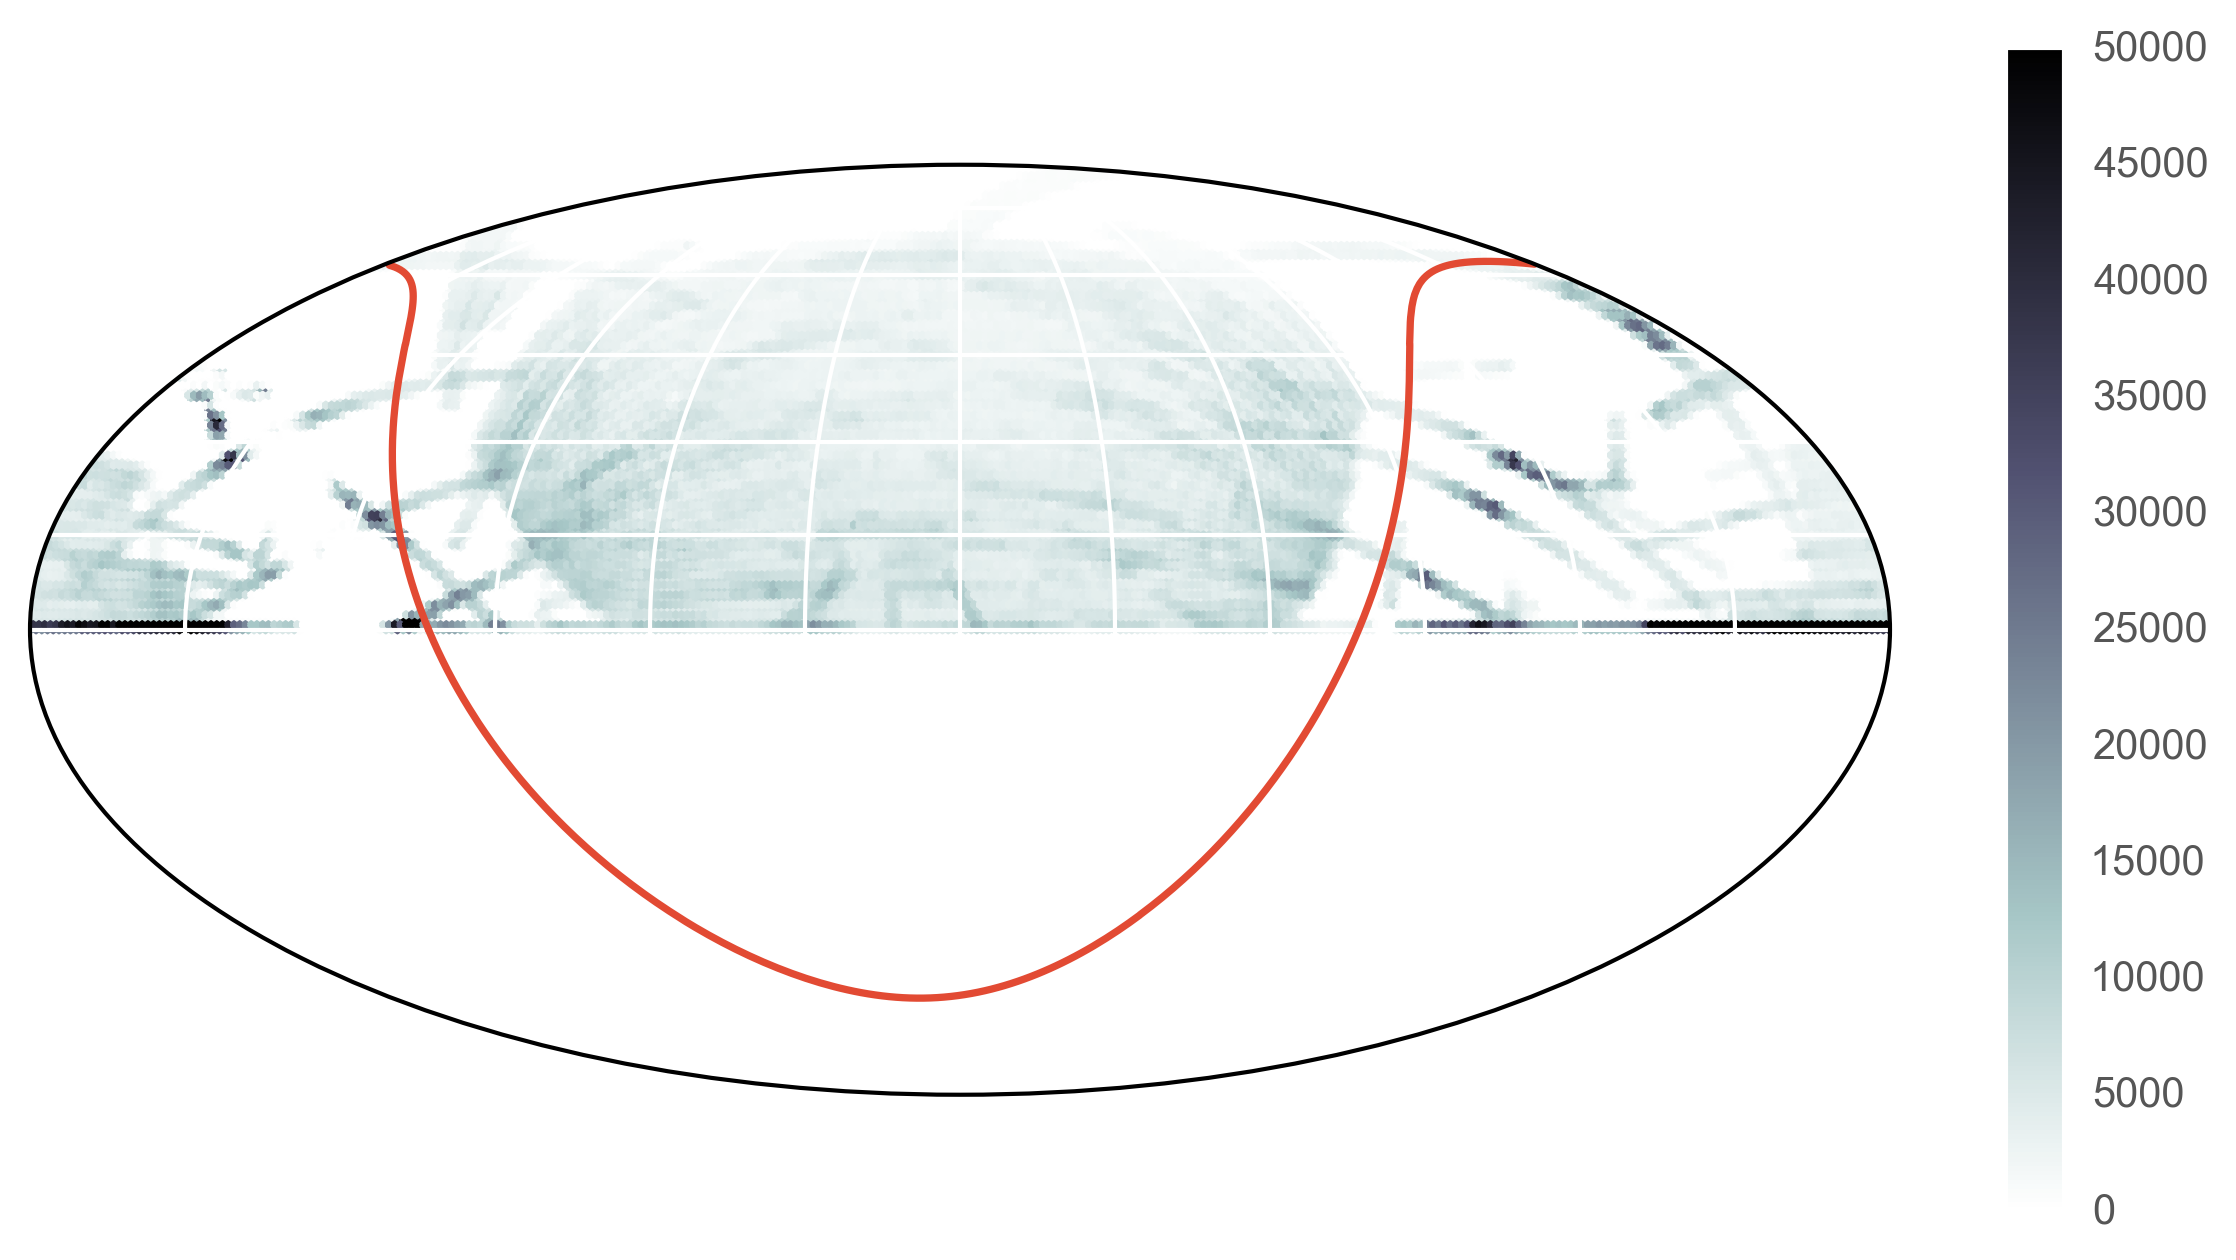
\includegraphics[width=0.75\linewidth]{figures/map_prediction_forest_quasars}
		\caption{Distribution of quasars.}
		\label{fig:random3}
	\end{subfigure}
	\caption{Map of predicted labels using random forest.}
	\label{fig:forest}
\end{figure}


%%% Local Variables: 
%%% mode: latex
%%% TeX-master: "thesis"
%%% End: 
